\documentclass{article}
\documentclass{article}

\usepackage{comment}
\usepackage[english]{isodate}
\usepackage{graphicx}
\usepackage[margin=1in]{geometry}
\usepackage{siunitx}
\usepackage{paracol}
\usepackage{enumitem}
\usepackage{bbm}
\usepackage[utf8]{inputenc}
\usepackage[T1]{fontenc}
\usepackage[bookmarks=true]{hyperref}
\usepackage{bookmark}
\usepackage{pdfpages} %\includepdf[pages={1}]{myfile.pdf}

\usepackage{amsmath}
\usepackage{ amssymb }
\usepackage{amsthm}
\usepackage{mdsymbol}%for perp with two bars

\usepackage{mathtools,xparse}
\newtheorem{theorem}{Theorem}

\DeclarePairedDelimiter{\abs}{\lvert}{\rvert}
\DeclarePairedDelimiter{\norm}{\lVert}{\rVert}

\newcommand{\E}{\mathbb{E}}
\newcommand{\Var}{\mathrm{Var}}
\newcommand{\Cov}{\mathrm{Cov}}
\newcommand\given[1][]{\:#1\vert\:}


\sisetup{output-decimal-marker = {,}}
\newcommand*{\ft}[1]{_\mathrm{#1}} 
\newcommand*{\dd}{\mathop{}\!\mathrm{d}}
\newcommand*{\tran}{^{\mkern-1.5mu\mathsf{T}}}%transpose of matrix
\newcommand{\trace}{\mathrm{trace}}

%%new
\newcommand{\tab}{\hspace{.2\textwidth}}
%\newcommand{\span}{\mathrm{Span}}
\renewcommand{\baselinestretch}{1.5}



%%%indenting
\newlength\tindent
\setlength{\tindent}{\parindent}
\setlength{\parindent}{0pt}
\renewcommand{\indent}{\hspace*{\tindent}}


\usepackage{enumitem}
\usepackage{times}
\usepackage{graphicx} % more modern
\usepackage{subfigure} 
\usepackage{natbib}
\usepackage{algorithm}
\usepackage{algorithmic}
\usepackage{hyperref}
\newcommand{\theHalgorithm}{\arabic{algorithm}}
\usepackage[accepted]{icml2016}

\usepackage{comment}
\newcommand{\compresslist}{
  \setlength{\itemsep}{1pt}
  \setlength{\parskip}{0pt}
  \setlength{\parsep}{0pt}}

%\yrcite{} if named otherwise \cite
\begin{document} 
\icmltitlerunning{LSTM}
\twocolumn[
\icmltitle{LSTM for Text Generation and Classsification}
\icmlauthor{Frédéric Boileau}{frederic.boileau@umontreal.ca}
\icmlauthor{Jimmy Leroux}{jimmy.leroux@umontreal.ca}
\icmlauthor{Nicolas Laliberté}{nicolas.laliberte@umontreal.ca}
\vskip 0.3in
]

\begin{abstract} 
In the context of our project for the IFT6269-A2018 we have investigated the
different available models for the generation and classification of natural
text data.  While we were initially interested in fully probabilistic models
such as Hidden Markov Models (HMM), a quick review of the contemporary
literature on the topic of pattern recognition on sequences made it clear that
neural networks (NN) provided the better toolset. In the end we implemented two
Long Short-Term Memory networks, for generation and classification respectively
which we trained on subsequences of some corpora of prose fiction. Despite the
rather coarse nature of our implementation the generators were able to produce
legible and decently structured text which reflected the material used for
training; in the style of the writing for example. The classifier reported 
excellent metrics however there are several interesting questions as to
what overfitting consists of when classifying prose fiction. The most
obvious is the one of proper nouns, but others such as temporal markers
are more subtle. The solutions to be decided with some context of the
intent of the task, so as to be the answer to a well-defined question.

\end{abstract} 

\medskip
\section{Introduction}
Hidden Markov Models used to be the go-to probabilistic tool to reason about
sequential data; the Markov assumption however proves to often be unreasonably
strong. Adding links to form higher order chains is not a scalable solution as
the computationnal complexity grows exponentially in the order of the chain.
Recurrent Neural Networks (RNN) constitute a family of neural network
architectures specialized to process sequential data which can forfeit
Markovian assumptions while remaining tractable.  RNNs can track longer range
dependencies while staying tractable by leveraging the simple idea of sharing
parameters across the model \cite{deeplearning}.  Concretely this means adding
loops to the hidden units of the neural network.  RNNs have been successfully
used in diverse domains for generating sequences such as music and text
\cite{gravesGenerating}.  Despite the aforementionned features, naive RNNs
suffer from the fact that the influence of some input to the hidden layer
either decays or blows up exponentially in time, a phenomenon reffered to in
the literature as the \textit{vanishing gradient problem}.  The cost of
abandonning probabilistic models such as the HMM in favor of neural networks is
the loss of a fully probabilistic interpretation. There has recently been an
increased interest into finding reasonable probabilistic interpretaions to
RNNs, see for example \cite{inter}. On the other hand the very existence of
some monolithic notion of ``interpretability'' has been recently questionned,
see \cite{mythos} for a philosophically inclined take on the question.

\section{Neural Networks Archicture}
\subsection{RNN and the Vanishing Gradient}
\begin{center}
    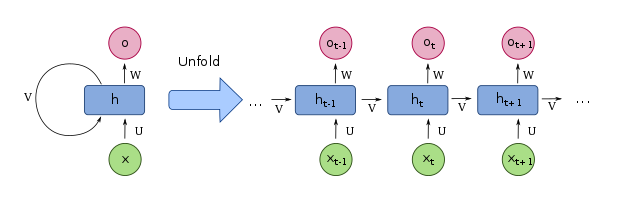
\includegraphics[width=\columnwidth]{RNN.png}
\end{center}
\begin{equation*}
    h_t = \sigma(U x_t + V h_{(t-1)} + b_h)
    \quad o_t = \text{softmax}(W h_t + b_o)
\end{equation*}
Where $ U$, $V$ and $W$ are weights matrix and the vectors $b$ are bias
parameters. Consider the gradient of $o_{t + \delta}$ with respect
to $h_t$. Applying the chain rule according to the graph above we get:

\begin{equation*}
  \nabla_{h_t} o_{t + \delta} = \left( \prod_{k = t+1}^{t+\delta} V^T
  \text{diag}(1 - h^2_k) \right)\nabla_{h_{t + \delta}}o_{t + \delta}.
\end{equation*}

Thus, as $\delta$ grows, the gradient grows exponentially with $V$. If $V$ is
small or large then the gradient will either vanish or explode. A myriad
of solutions exist such as regularization through weight noise, the Long Short
Term Memory architecture tries to tackle this issue on a higher level than
regularization.
\subsection{LSTM Architecture}
To go from a RNN to a LSTM we replace hidden units with components known as
\textit{memory cells}. Our presentation and notation follows \cite{revieww}.
\begin{center}
    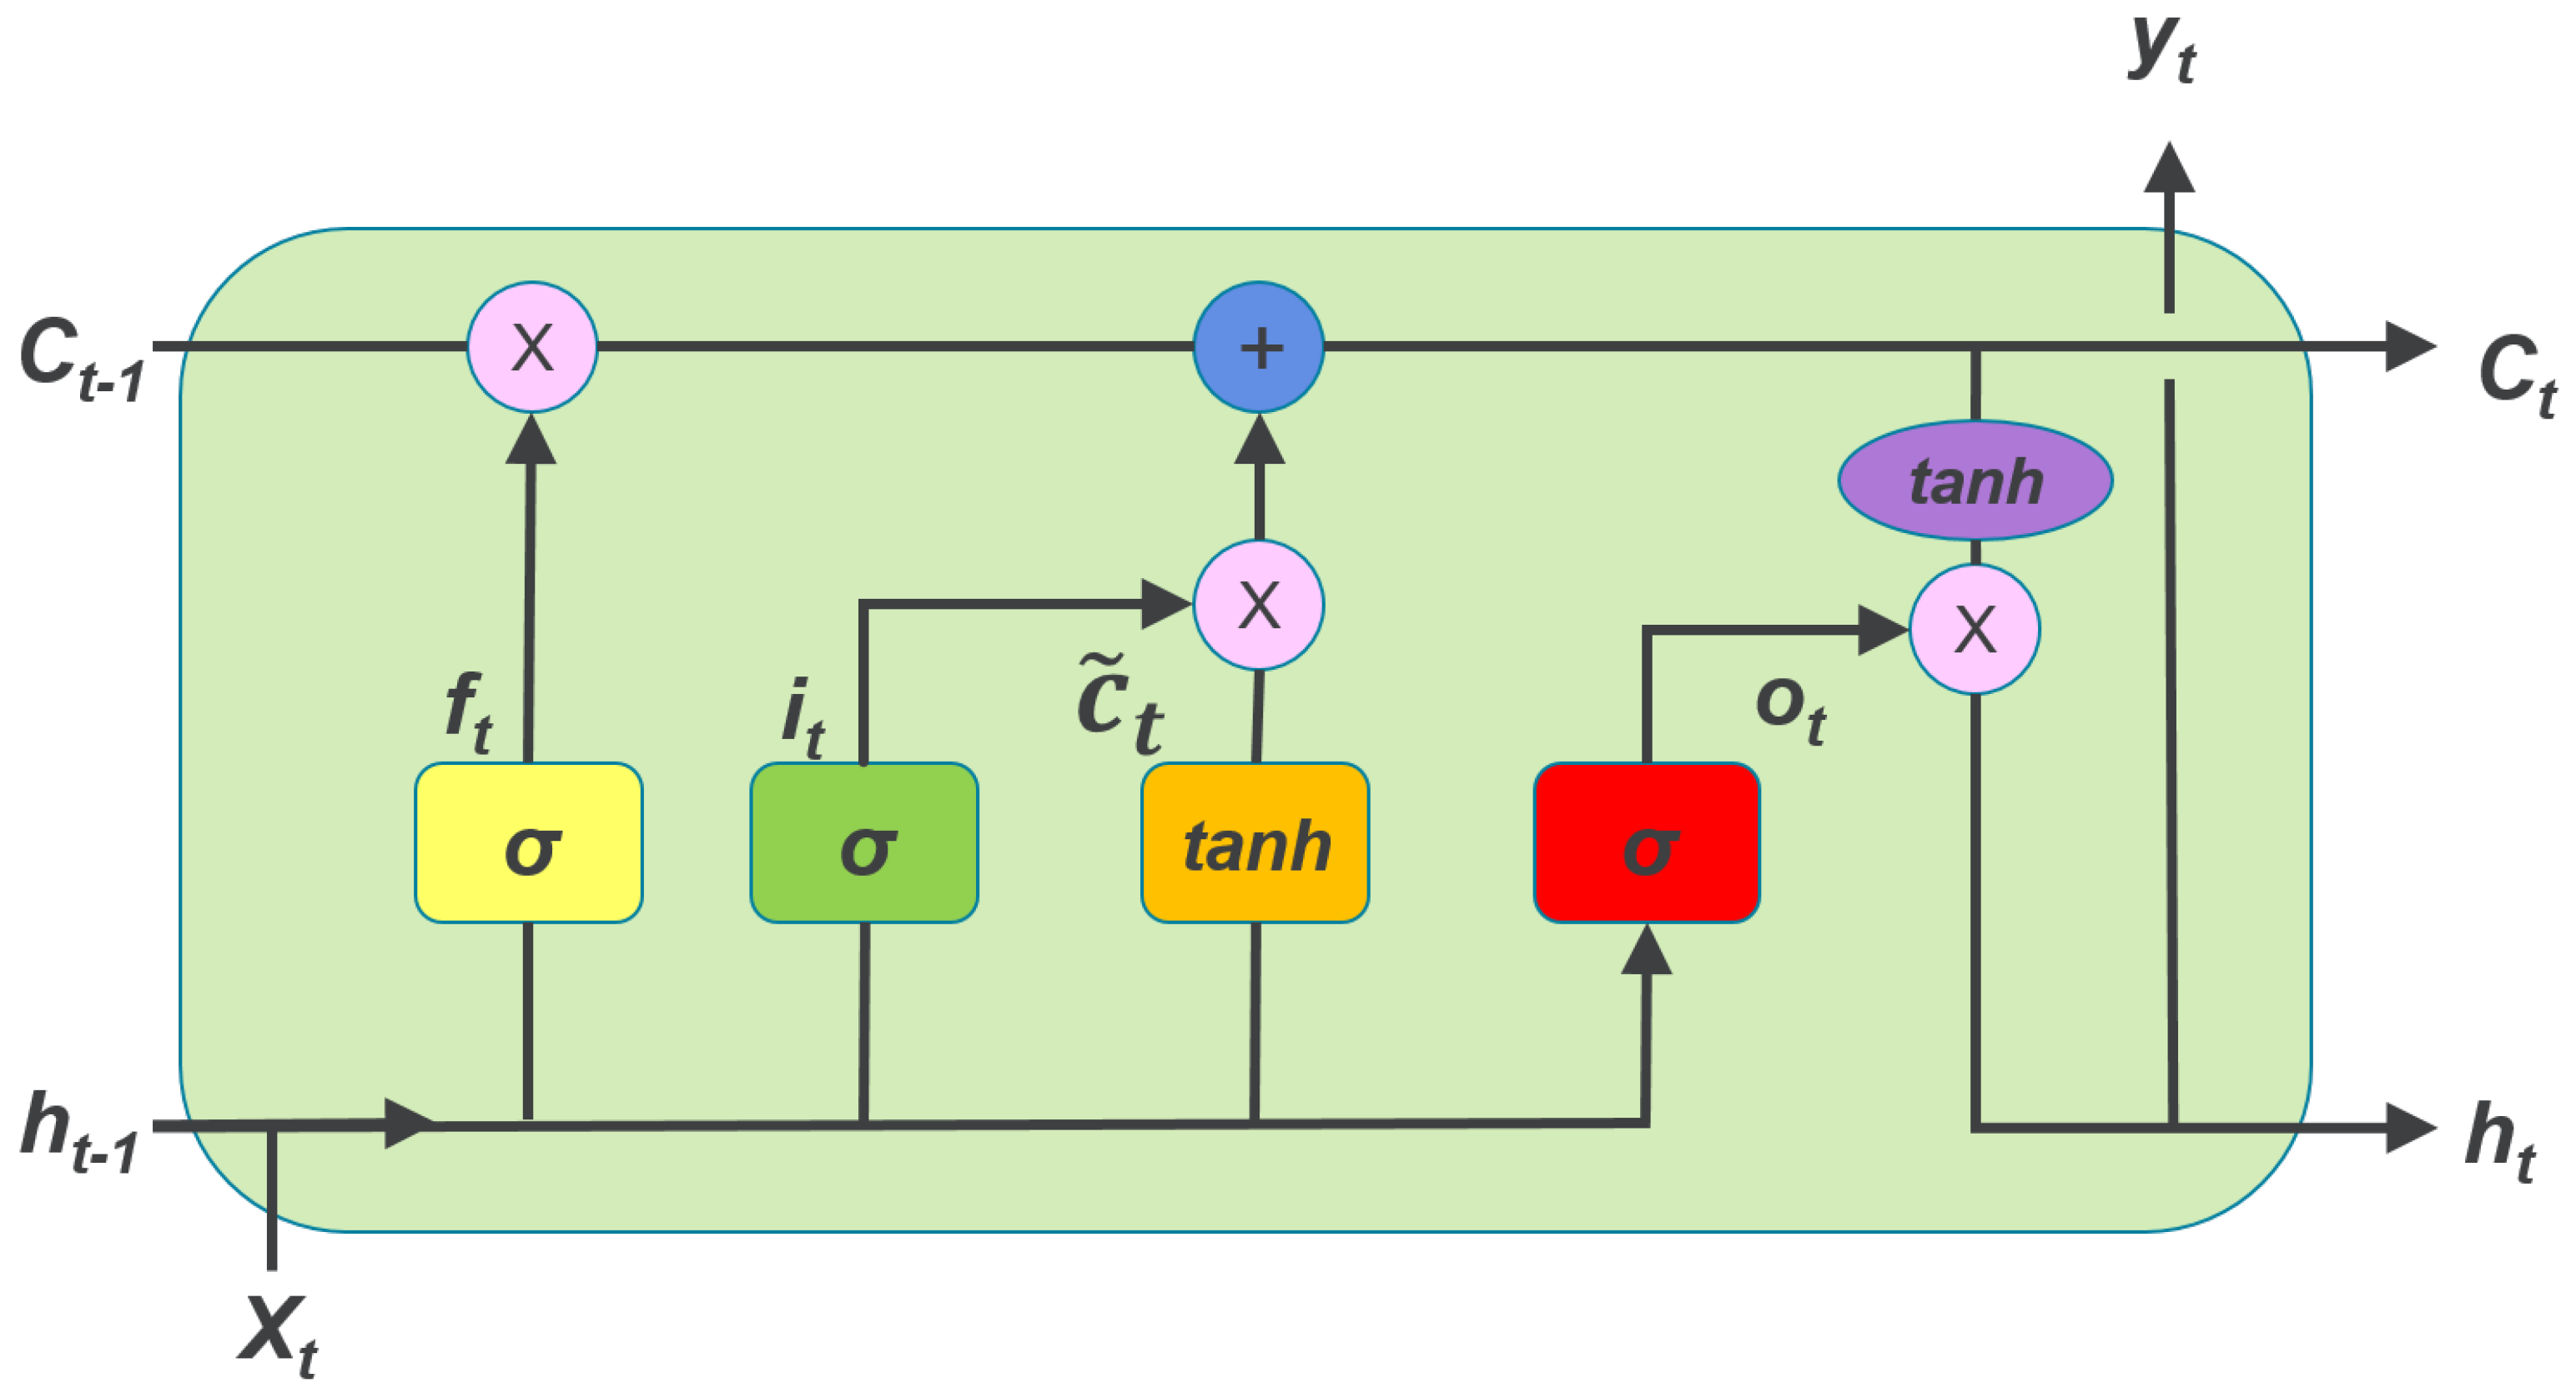
\includegraphics[width =\columnwidth]{lstm.png}
\end{center}

Intuitively, RNNs have \textit{long-term memory} in the form of matrix weights,
they change during the training; encoding through training some general
knowledge about the data. They also have \textit{short-term memory} in the form
of activation passing from each node to successive ones. The memory cell
introduced in the LSTM model formalizes those notions and provides a framework
to control their impact on the internal representation of the network.
\begin{center}
    \begin{itemize}
    \item $f_t, i_t, o_t$: Respectively forget, input and output gates.
        \begin{itemize}
            \normalsize
            \item Sigmoidal units activated through  $x_t$ (current input) and
                $h_{t-1}$ (past hidden unit output) \item $f_t$ controls the
                recursive flow
            \item $i_t$ and $o_t$ control the input and output flow
                respectively
            \item $h_t = o_t \odot \tanh(c_t)$ where $\odot$ denotes element
                wise multiplication.
        \end{itemize}
    \item $c_t = \mathbf{f_t \odot c_{t-1}} + i_t \odot \tilde{c}_t$: The cell
    which has a self-connected edge with a fixed unit weight, thereby delegating
    control of recursion to the gate
    \end{itemize}
\end{center}
\section{Implementation}
Four text sequences (referred to as datasets later on) were used for training:
excerpts from Shakespeare' plays, books of the Harry Potter and Lord of the
Ring series and a list of popular quotes.  All in English and ASCII encoded.
Punctuation and structure was left unprocessed.  Each dataset was split in
sequences of 50 tokens (i.e.  ``words'') and a dictionnary was built from the
complete input ($\approx 60k$ unique tokens), defining the input space for the
networks.  Vector encoding of this space was used through an embedding layer
mapping the words to a real vector space of dimension 256.  Available
embeddings such as \textit{word2vec} and \textit{glove} were initally used but
proved to be more cumbersome than our own trained version.  Five LSTM networks
were trained with the above, Four \textit{generators} and a
\textit{classifier}. Training was achieved at ``word'' level (strings tokenized
by whitespace). Character level had been previsously envisionned for the rest
of the project as it is more flexible and can \textit{learn new words and
structural information}\cite{gravesGenerating} for the generators). Despite
this we kept the training at word level for multiple reasons, the primary one
being robustness towards unicode characters which might vary between versions
of the text available and the second one being speed of convergence. 

To generate the sequences the trained models were initialized with a random word
drawn from the dictionary and the most likely next word was fed back in the network
until the desired sequence length was reached. 1000 sequences (250 per model) were
generated. The classifier was then used to automatically estimate which
dataset (or model, equivalently) was used for its generation, thereby giving us
some ``metric'' of the quality of the data; expecting data generated from the
Shakespeare trained model to consistenly differ from the data ``generated by
Harry Potter''.
\clearpage
\section{Empirical Results}
\begin{figure}[ht]
\vskip 0.2in
\begin{center}
\centerline{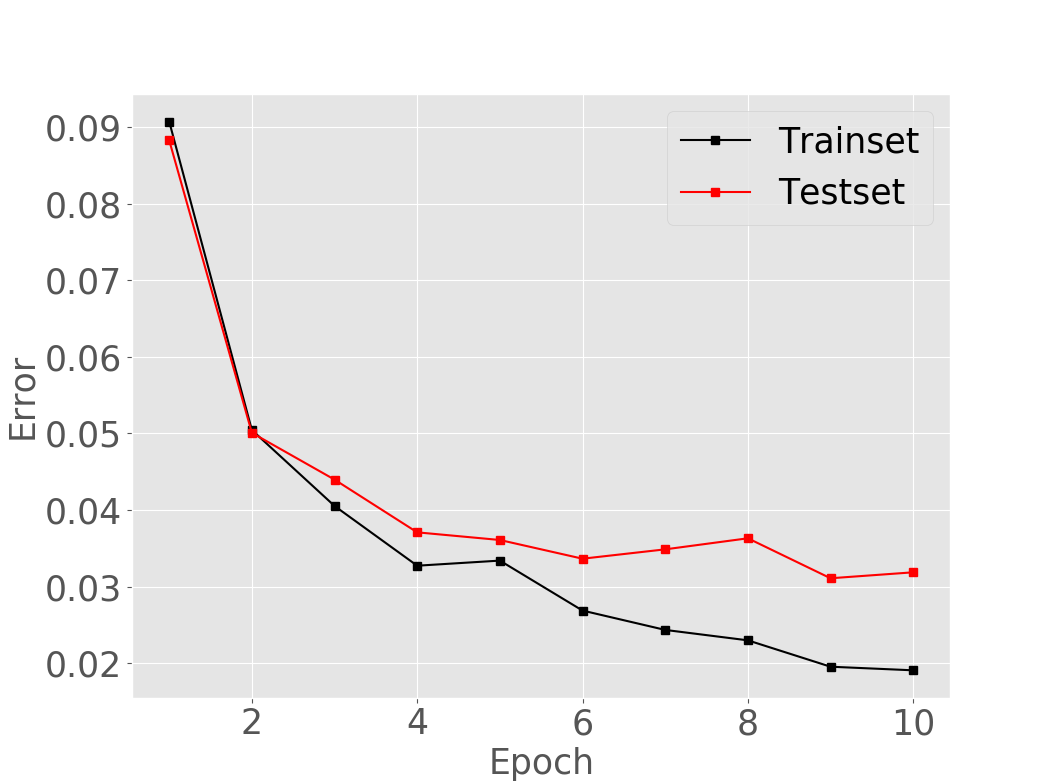
\includegraphics[width=\columnwidth]{classerror}}
\caption{Classification error on train/test set.}
\end{center}
\vskip -0.2in
\end{figure} 

Training trough minimization of the cross-entropy loss, which is equivalent to
\textit{perplexity}; the standard metric for language
modeling \cite{gravesGenerating}.
\begin{figure}[htbp!]
\begin{tabular}{|l|l|c|}
\hline
Dataset & BPC & Perplexity \\
\hline
Harry Potter & 1.00 & 33 \\
LOTR & 1.02 & 35 \\
Random quotes & 1.10 & 45 \\
Shakespeare & 0.94 & 26\\
\hline
\end{tabular}
\end{figure}

Examples of generated quotes:
\begin{itemize}\compresslist
    \item `` well , we ' ll do it with a wand , '' said hermione . `` really ?
      '' said harry , looking at each other .
    \item  what looked about this
      way , the black citadel , was far from the
          darkness , the ring was heard , but the sea big was big , and a great
          ring was in his battle .
    \item failure is a beginning of love and a family which comes from god .
    \item  '' that now my mind shall screens his music , '' '' and i to give
      thee my vulgar heaven , '' '' i am your brother .
\end{itemize}
\section{Conclusion and Further Work}
\section{Citations and References} 

\bibliography{example_paper}
\bibliographystyle{icml2016}

\end{document} 


%examples
\begin{figure}[ht]
\vskip 0.2in
\begin{center}
\centerline{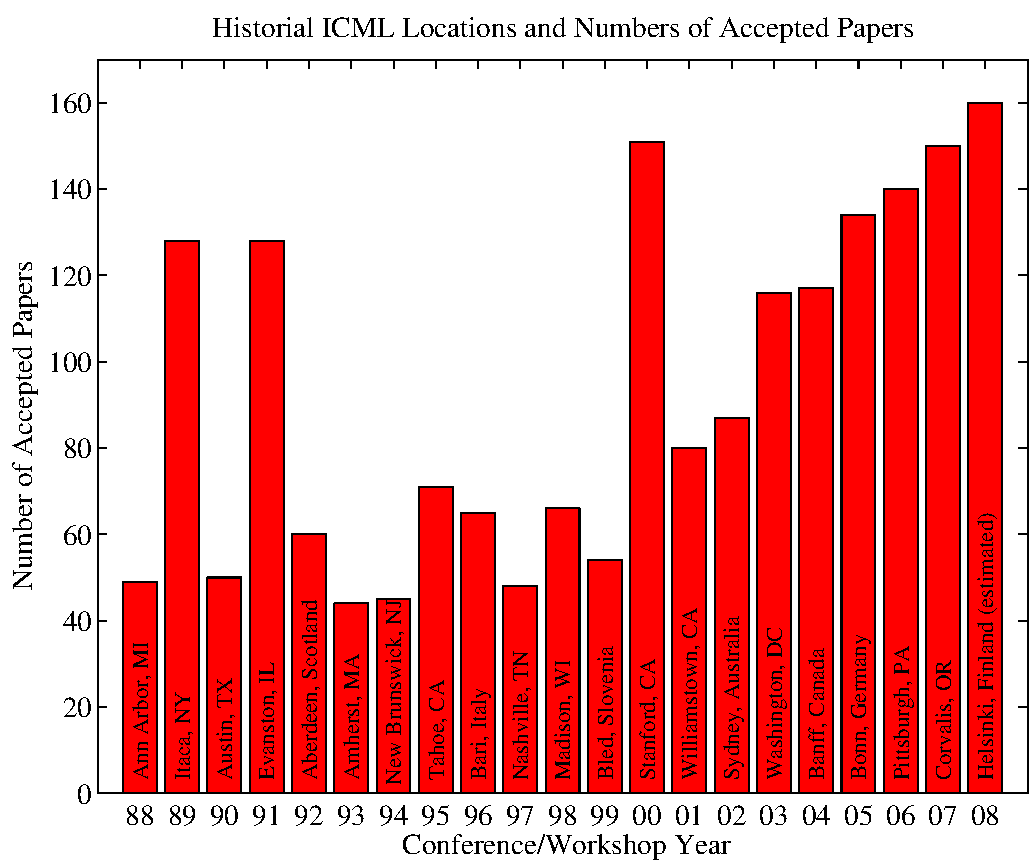
\includegraphics[width=\columnwidth]{icml_numpapers}}
\caption{}
\label{icml-historical}
\end{center}
\vskip -0.2in
\end{figure} 

\begin{algorithm}[tb]
   \caption{Bubble Sort}
   \label{alg:example}
\begin{algorithmic}
   \STATE {\bfseries Input:} data $x_i$, size $m$
   \REPEAT
   \STATE Initialize $noChange = true$.
   \FOR{$i=1$ {\bfseries to} $m-1$}
   \IF{$x_i > x_{i+1}$} 
   \STATE Swap $x_i$ and $x_{i+1}$
   \STATE $noChange = false$
   \ENDIF
   \ENDFOR
   \UNTIL{$noChange$ is $true$}
\end{algorithmic}
\end{algorithm}
 
\begin{table}[t]
\caption{Classification accuracies for naive Bayes and flexible 
Bayes on various data sets.}
\label{sample-table}
\vskip 0.15in
\begin{center}
\begin{small}
\begin{sc}
\begin{tabular}{lcccr}
\hline
\abovespace\belowspace
Data set & Naive & Flexible & Better? \\
\hline
\abovespace
Breast    & 95.9$\pm$ 0.2& 96.7$\pm$ 0.2& $\surd$ \\
Cleveland & 83.3$\pm$ 0.6& 80.0$\pm$ 0.6& $\times$\\
Glass2    & 61.9$\pm$ 1.4& 83.8$\pm$ 0.7& $\surd$ \\
Credit    & 74.8$\pm$ 0.5& 78.3$\pm$ 0.6&         \\
Horse     & 73.3$\pm$ 0.9& 69.7$\pm$ 1.0& $\times$\\
Meta      & 67.1$\pm$ 0.6& 76.5$\pm$ 0.5& $\surd$ \\
Pima      & 75.1$\pm$ 0.6& 73.9$\pm$ 0.5&         \\
\belowspace
Vehicle   & 44.9$\pm$ 0.6& 61.5$\pm$ 0.4& $\surd$ \\
\hline
\end{tabular}
\end{sc}
\end{small}
\end{center}
\vskip -0.1in
\end{table}
